%
%    This program is free software; you can redistribute it and/or modify
%    it under the terms of the GNU General Public License as published by
%    the Free Software Foundation; either version 2 of the License, or
%    (at your option) any later version.
%
%    This program is distributed in the hope that it will be useful,
%    but WITHOUT ANY WARRANTY; without even the implied warranty of
%    MERCHANTABILITY or FITNESS FOR A PARTICULAR PURPOSE.  See the
%    GNU General Public License for more details.
%
%    You should have received a copy of the GNU General Public License
%    along with this program; if not, write to the Free Software
%    Foundation, Inc., 675 Mass Ave, Cambridge, MA 02139, USA.
%

% Version: $Revision$

The ArffViewer is a little tool for viewing ARFF files in a tabular format. The advantage of this kind of display over the file representation is, that attribute name, type and data are directly associated in columns and not separated in defintion and data part. But the viewer is not only limited to viewing multiple files at once, but also provides simple editing functionality, like sorting and deleting.

\begin{center}
	\epsfig{file=images/arffviewer/arffviewer_main.eps,height=12cm,angle=-90}
\end{center}

\newpage
\section{Menus}
The ArffViewer offers most of its functionality either through the main menu or via popups (table header and table cells). 

Short description of the available menus:
\begin{itemize}
	\item \textbf{File} \\
		\epsfig{file=images/arffviewer/arffviewer_menu_file.eps,height=4cm} \\
		contains options for opening and closing files, as well as viewing properties about the current file.
	\item \textbf{Edit} \\
		\epsfig{file=images/arffviewer/arffviewer_menu_edit.eps,height=4cm} \\
		allows one to delete attributes/instances, rename attributes, choose a new class attribute, search for certain values in the data and of course undo the modifications.
	\item \textbf{View} \\
		\epsfig{file=images/arffviewer/arffviewer_menu_view.eps,height=4cm,angle=-90} \\
		brings either the chosen attribute into view or displays all the values of an attribute. 
\end{itemize}

After opening a file, by default, the column widths are optimized based on the attribute name and not the content. This is to ensure that overlong cells do not force an enormously wide table, which the user has to reduce with quite some effort. 

\newpage
In the following, screenshots of the table popups:
\begin{center}
	\epsfig{file=images/arffviewer/arffviewer_tableheader_popup.eps,height=12cm,angle=-90}
\end{center}

\begin{center}
	\epsfig{file=images/arffviewer/arffviewer_table_popup.eps,height=12cm,angle=-90}
\end{center}


\newpage
\section{Editing}
Besides the first column, which is the instance index, all cells in the table are editable. Nominal values can be easily modified via dropdown lists, numeric values are edited directly.

\begin{center}
	\epsfig{file=images/arffviewer/arffviewer_editing_nominal.eps,height=12cm,angle=-90}
\end{center}

\newpage
For convenience, it is possible to sort the view based on a column (the underlying data is NOT changed; via Edit/Sort data one can sort the data permanently). This enables one to look for specific values, e.g., missing values. To better distinguish missing values from empty cells, the background of cells with missing values is colored grey.

\begin{center}
	\epsfig{file=images/arffviewer/arffviewer_sort_view.eps,height=12cm,angle=-90}
\end{center}
